% --- APPENDICES ---
\newpage
\appendix

\chapter{Supplementary Materials}
\label{sec:supplementary}

This appendix presents supplementary spatial figures referenced in Chapter~\ref{sec:spatial_analysis}. Choropleth and scatter plots use Austrian administrative boundaries from \cite{igismap_austria_shapefile} and regional socioeconomic indicators from \cite{statistik_atlas,ec_health_monitoring_2002}.

\section{Supplementary Figures: Socioeconomic Factors}

\begin{figure}[H]
    \centering
    \begin{subfigure}[b]{0.48\textwidth}
        \centering
        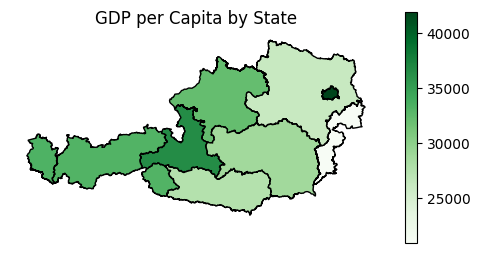
\includegraphics[width=\textwidth]{figures/gdpbystate.png}
        \caption{Regional GDP per capita by Austrian state.}
        \label{fig:gdp_by_state}
    \end{subfigure}
    \hfill
    \begin{subfigure}[b]{0.48\textwidth}
        \centering
        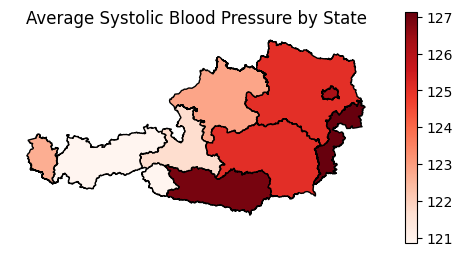
\includegraphics[width=\textwidth]{figures/avgsysbpbystate.png}
        \caption{Average systolic blood pressure by state.}
        \label{fig:avg_sys_bp_by_state_sidebyside}
    \end{subfigure}
    \caption{Comparison of GDP per capita (left) and average systolic blood pressure (right) across Austrian states based on the health screening dataset. These plots illustrate potential regional variation in socioeconomic status and cardiovascular health.}
    \label{fig:gdp_and_bp_sidebyside}
\end{figure}
 
\begin{figure}[H]
    \centering
    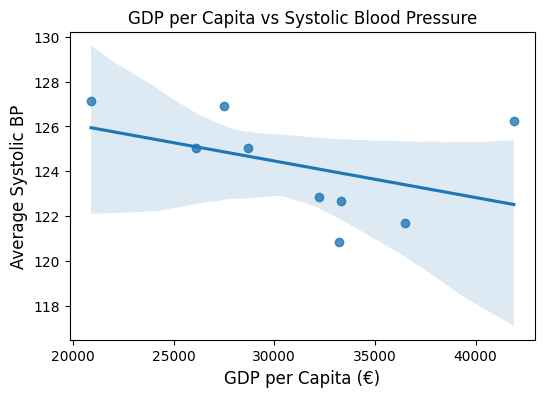
\includegraphics[width=0.7\textwidth]{figures/gdpvssysbp.png}
    \caption{Scatter plot of regional GDP per capita versus mean systolic blood pressure by Austrian state. Each point represents one state from the health screening dataset, illustrating the absence of a strong regional association between economic prosperity and average systolic blood pressure.}
    \label{fig:gdp_vs_sysbp}
\end{figure}

\begin{figure}[H]
    \centering
    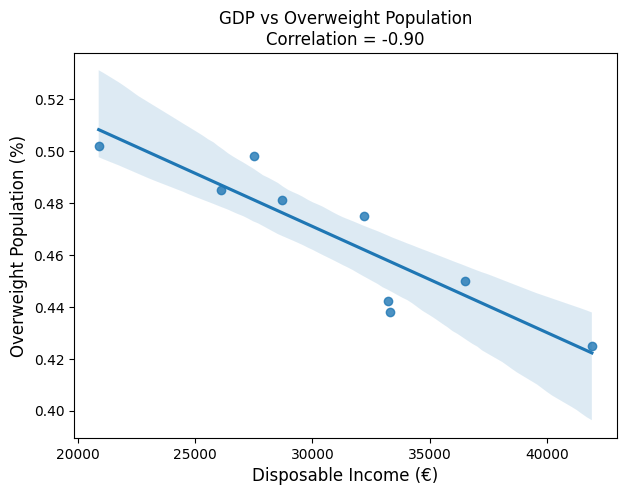
\includegraphics[width=0.7\textwidth]{figures/gdpvsobesity.png}
    \caption{Scatter plot of regional GDP per capita versus overweight prevalence (proportion of population with BMI $\geq 25$) by Austrian state. Each point represents one state, showing the strong negative association between economic prosperity and population-level overweight prevalence observed in the health screening dataset and public health statistics.}
    \label{fig:gdp_vs_obesity}
\end{figure}

\begin{figure}[H]
    \centering
    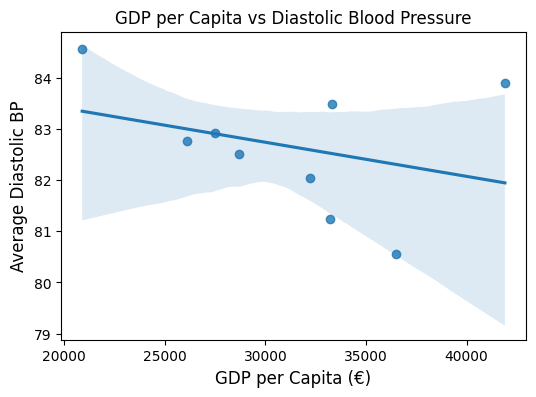
\includegraphics[width=0.7\textwidth]{figures/gdpvsdiabp.png}
    \caption{Scatter plot of regional GDP per capita versus mean diastolic blood pressure by Austrian state. Each point represents one state, illustrating whether regional economic prosperity is associated with variation in average diastolic blood pressure across Austria.}
    \label{fig:gdp_vs_diabp}
\end{figure}

\begin{figure}[H]
    \centering
    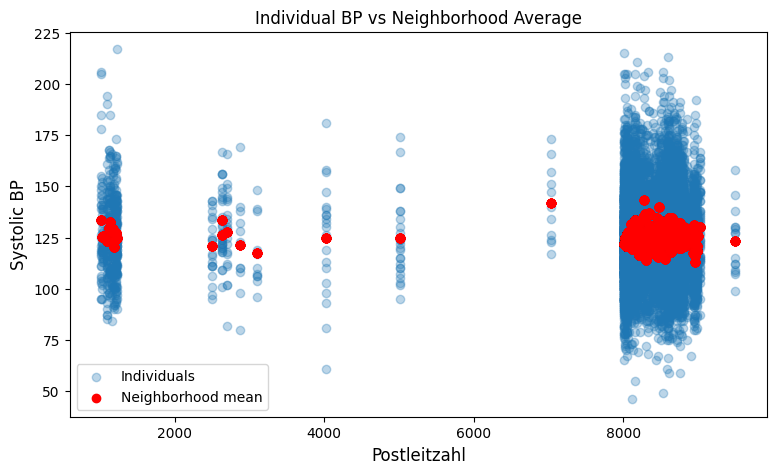
\includegraphics[width=0.7\textwidth]{figures/bpvsneap.png}
    \caption{Scatter plot of neighbourhood mean systolic blood pressure versus individual diastolic blood pressure. Each point represents an individual's measurement, coloured or grouped by neighbourhood (postal code). This figure visualises the contextual relationship explored in the NEAP regression analysis, supporting the modest but non-negligible association between neighbourhood systolic averages and individual diastolic outcomes.}
    \label{fig:bp_vs_neap}
\end{figure}


\chapter{AI Usage Declaration}
\label{sec:appendix}

\emph{I declare that I used ChatGPT (OpenAI GPT-4) to assist with structuring the report, 
improving clarity of explanations, and polishing the 
academic writing of several sections. In addition it was used to refactor, add inline documentation and to improve the readability of the code.}

\emph{In addition cursor agents were used to suggest improvements in section organization, 
to help draft interpretations of figures and tables based on results I had already generated, 
refining \LaTeX{} formatting, and to assist in wording the discussion and future work sections.}

\emph{The design of the research question, data preprocessing, feature engineering, 
implementation of the code and models, experimental setup, 
statistical evaluation are entirely my own work. All final decisions regarding methodology, analysis, and conclusions were made independently by me.}
